\documentclass{beamer}

\newcommand{\lesson}{OOP Case Studies: Collections and JavaFX}

\newcommand{\course}{Introduction to Object-Oriented Programming}
\subject{\course}
\title[\lesson]{\course}
\subtitle{\lesson}

\author[CS 1331]
{Christopher Simpkins \\\texttt{chris.simpkins@gatech.edu}}
\institute[Georgia Tech]

\date[]{}

\newcommand{\link}[2]{\href{#1}{\textcolor{blue}{\underline{#2}}}}
\newcommand{\code}{http://www.cc.gatech.edu/~simpkins/teaching/gatech/cs1331/code}

\usepackage{colortbl}

% If you have a file called "university-logo-filename.xxx", where xxx
% is a graphic format that can be processed by latex or pdflatex,
% resp., then you can add a logo as follows:

% \pgfdeclareimage[width=0.6in]{coc-logo}{cc_2012_logo}
% \logo{\pgfuseimage{coc-logo}}

\mode<presentation>
{
  \usetheme{Berlin}
  \useoutertheme{infolines}

  % or ...

 \setbeamercovered{transparent}
  % or whatever (possibly just delete it)
}

\usepackage{tikz}
% Optional PGF libraries
\usepackage{pgflibraryarrows}
\usepackage{pgflibrarysnakes}
\usepackage{pgfplots}
\usepackage{fancybox}
\usepackage{listings}
\usepackage[abbr]{harvard}
\usepackage{hyperref}
\hypersetup{colorlinks=true,urlcolor=blue}
\usepackage[english]{babel}
% or whatever

\usepackage[latin1]{inputenc}
% or whatever

\usepackage{times}
\usepackage[T1]{fontenc}
% Or whatever. Note that the encoding and the font should match. If T1
% does not look nice, try deleting the line with the fontenc.


\usepackage{listings}

% "define" Scala
\lstdefinelanguage{scala}{
  morekeywords={abstract,case,catch,class,def,%
    do,else,extends,false,final,finally,%
    for,if,implicit,import,match,mixin,%
    new,null,object,override,package,%
    private,protected,requires,return,sealed,%
    super,this,throw,trait,true,try,%
    type,val,var,while,with,yield},
  otherkeywords={=>,<-,<\%,<:,>:,\#,@},
  sensitive=true,
  morecomment=[l]{//},
  morecomment=[n]{/*}{*/},
  morestring=[b]",
  morestring=[b]',
  morestring=[b]""",
}

\usepackage{color}
\definecolor{dkgreen}{rgb}{0,0.6,0}
\definecolor{gray}{rgb}{0.5,0.5,0.5}
\definecolor{mauve}{rgb}{0.58,0,0.82}

% Default settings for code listings
\lstset{frame=tb,
  language=scala,
  aboveskip=2mm,
  belowskip=2mm,
  showstringspaces=false,
  columns=flexible,
  basicstyle={\scriptsize\ttfamily},
  numbers=none,
  numberstyle=\tiny\color{gray},
  keywordstyle=\color{blue},
  commentstyle=\color{dkgreen},
  stringstyle=\color{mauve},
  frame=single,
  breaklines=true,
  breakatwhitespace=true,
  keepspaces=true
  %tabsize=3
}


% If you wish to uncover everything in a step-wise fashion, uncomment
% the following command:

% \beamerdefaultoverlayspecification{<+->}


\begin{document}

\begin{frame}
  \titlepage
\end{frame}

%------------------------------------------------------------------------
\begin{frame}[fragile]{The Collections Framework}

\begin{center}
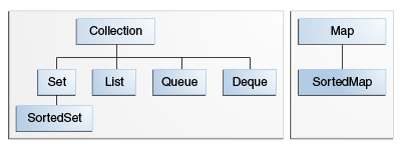
\includegraphics[width=4in]{colls-coreInterfaces.png}
\end{center}

\begin{itemize}
\item A {\it collection} is an object that represents a group of objects.
\item The collections framework allows different kinds of collections to be dealt with in an implementation-independent manner.
\end{itemize}


\end{frame}
%------------------------------------------------------------------------

%------------------------------------------------------------------------
\begin{frame}[fragile]{Collection Framework Components}

The Java collections framework consists of:
\begin{itemize}
\item Collection interfaces representing different types of collections ({\tt Set}, {\tt List}, etc)
\item General purpose implementations (like {\tt ArrayList} or {\tt HashSet})
\item Abstract implementations to support custom implementations
\item Algorithms defined in static utility methods that operate on collections (like {\tt Collections.sort(List<T> list)})
\item Infrastructure interfaces that support collections (like {\tt Iterator})
\end{itemize}

\end{frame}
%------------------------------------------------------------------------

%------------------------------------------------------------------------
\begin{frame}[fragile]{{\tt ArrayList} Basics}


Create an {\tt ArrayList} with operator {\tt new}:
\begin{lstlisting}[language=Java]
  ArrayList tasks = new ArrayList();
\end{lstlisting}
Add items with {\tt add()}:
\begin{lstlisting}[language=Java]
  tasks.add("Eat");
  tasks.add("Sleep");
  tasks.add("Code");
\end{lstlisting}
Traverse with for-each loop:
\begin{lstlisting}[language=Java]
  for (Object task: tasks) {
      System.out.println(task);
  }
\end{lstlisting}

Note that the for-each loop implicitly uses an iterator.

\end{frame}
%------------------------------------------------------------------------

%------------------------------------------------------------------------
\begin{frame}[fragile]{Using Iterators}


Iterators are objects that provide access to the elements in a collection.  In Java iterators are represented by the {\tt Iterator} interface, which contains three methods:
\begin{itemize}
\item {\tt hasNext()} returns true if the iteration has more elements.
\item {\tt next()} returns the next element in the iteration.
\item {\tt remove()} removes from the underlying collection the last element returned by the iterator (optional operation).
\end{itemize}

The most basic and common use of an iterator is to traverse a collection (visit all the elements in a collection):
\begin{lstlisting}[language=Java]
ArrayList tasks = new ArrayList();
// ...
Iterator tasksIter = tasks.iterator();
while (tasksIter.hasNext()) {
    Object task = tasksIter.next();
    System.out.println(task);
}
\end{lstlisting}
See \link{\code/collections/ArrayListBasics.java}{ArrayListBasics.java} for more.

\end{frame}
%------------------------------------------------------------------------

%------------------------------------------------------------------------
\begin{frame}[fragile]{Defining Iterators}

\vspace{-.1in}
\begin{lstlisting}[language=Java]
public class DynamicArray<E> implements Iterable<E> {
    private class DynamicArrayIterator implements Iterator<E> {
        private int cursor = 0;
        public boolean hasNext() {
            return cursor <= DynamicArray.this.lastIndex;
        }
        public E next() {
            cursor++;
            return DynamicArray.this.get(cursor - 1);
        }
        public void remove() { DynamicArray.this.remove(cursor - 1); }
    }
    private Object[] elements;
    private int lastIndex;
    public DynamicArray(int capacity) {
        elements = new Object[capacity]; lastIndex = -1;
    }
    public Iterator iterator() { return new DynamicArrayIterator(); }
\end{lstlisting}
\vspace{-.1in}
See \link{\code/collections/DynamicArray.java}{DynamicArray.java} for examples.

\end{frame}
%------------------------------------------------------------------------

%------------------------------------------------------------------------
\begin{frame}[fragile]{The Iterable Interface}

The {\tt Iterable} interface has one abstract method, {\tt iterator}:

\begin{lstlisting}[language=Java]
public interface Iterable<T> {
    Iterator<T> iterator();
}
\end{lstlisting}

An instance of a class that implements {\tt Iterable} can be the target of a for-each loop.
\begin{lstlisting}[language=Java]
        DynamicArray<String> da = new DynamicArray<>(2);
        da.add("Stan");
        da.add("Kenny");
        da.add("Cartman");
        System.out.println("da contents:");
        for (String e: da) {
            System.out.println(e);
        }

\end{lstlisting}

\end{frame}
%------------------------------------------------------------------------


%------------------------------------------------------------------------
\begin{frame}[fragile]{Using Generics}


Supply a type argument in the angle brackets.  Read {\tt ArrayList<String>} as ``ArrayList of String''
\begin{lstlisting}[language=Java]
  ArrayList<String> strings = new ArrayList<String>();
  strings.add("Helluva"); strings.add("Engineer!");
\end{lstlisting}
If we try to add an object that isn't a {\tt String}, we get a compile error:
\begin{lstlisting}[language=Java]
  Integer BULL_DOG = Integer.MIN_VALUE;
  strings.add(BULL_DOG); // Won't compile
\end{lstlisting}

With a typed collection, we get autoboxing on insertion {\it and} retrieval:

\begin{lstlisting}[language=Java]
  ArrayList<Integer> ints = new ArrayList<>();
  ints.add(42);
  int num = ints.get(0);
\end{lstlisting}
Notice that we didn't need to supply the type parameter in the creation expression above.  Java inferred the type parameter from the declaration. (Note: this only works in Java 7 and above.)

See \link{\code/collections/ArrayListGenericsDemo.java}{ArrayListGenericsDemo.java} for examples.

\end{frame}
%------------------------------------------------------------------------

%------------------------------------------------------------------------
\begin{frame}[fragile]{{\tt Set}s}

A {\tt Set} is a collection with no duplicate elements (no two elements {\tt e1} and {\tt e2} for which {\tt e1.equals(e2)}) and in no particular order.  Given:
\begin{lstlisting}[language=Java]
List<String> nameList = Arrays.asList("Alan", "Ada", "Alan");
Set<String> nameSet = new HashSet<>(nameList);
System.out.println("nameSet: " + nameSet);
\end{lstlisting}
will print:
\begin{lstlisting}[language=Java]
nameSet: [Alan, Ada]
\end{lstlisting}

\end{frame}
%------------------------------------------------------------------------

%------------------------------------------------------------------------
\begin{frame}[fragile]{{\tt Map}s}

\vspace{-.05in}
A {\tt Map<K, V>} object maps keys of type {\tt K} to values of type {\tt V}.  The code:
\vspace{-.05in}
\begin{lstlisting}[language=Java]
  Map<String, String> capitals = new HashMap<>();
  capitals.put("Georgia", "Atlanta");
  capitals.put("Alabama", "Montgomery");
  capitals.put("Florida", "Tallahassee");
  for (String state: capitals.keySet()) {
      System.out.println("Capital of " + state + " is "
                         + capitals.get(state));
  }
\end{lstlisting}
\vspace{-.05in}
prints:
\vspace{-.05in}
\begin{lstlisting}[language=Java]
Capital of Georgia is Atlanta
Capital of Florida is Tallahassee
Capital of Alabama is Montgomery
\end{lstlisting}
\vspace{-.05in}
Note that the order of the keys differs from the order in which we added them.  The keys of a map are a {\tt Set}, so there can be no duplicates and order is not guaranteed.  If you {\tt put} a new value with the same key as an entry already in the map, that entry is overwritten with the new one.

\end{frame}
%------------------------------------------------------------------------


%------------------------------------------------------------------------
\begin{frame}[fragile]{Using {\tt Collections.sort(List<T> list)}}


The collections framework includes algorithms that operate on collections implemented as static methods of the {\tt Collections} class.  A good example is the {\tt sort} method:
\begin{lstlisting}[language=Java]
public static <T extends Comparable<? super T>> void sort(List<T> list)
\end{lstlisting}

\begin{itemize}
\item {\tt sort} uses the ``natural ordering'' of the list, that is, the ordering defined by {\tt Comparable}.
\item {\tt <? super T>} is a {\it type bound}.  It means ``some superclass of {\tt T}.''
\item The {\tt <T extends Comparable<? super T>>} means that the element type {\tt T} or some superclass of {\tt T} must implement {\tt Comparable}.
\end{itemize}

See \link{\code/collections/super-troopers/SortTroopers.java}{SortTroopers.java} for examples.

\end{frame}
%------------------------------------------------------------------------

%------------------------------------------------------------------------
\begin{frame}[fragile]{Can we {\tt Collections.sort(List<T> list)}?}

\vspace{-.05in}
Given the {\tt Collections} static method:
\begin{lstlisting}[language=Java]
public static <T extends Comparable<? super T>> void sort(List<T> list)
\end{lstlisting}
\vspace{-.05in}
And the classes:
\vspace{-.05in}
\begin{lstlisting}[language=Java]
public class Person implements Comparable<Person>
public class GtStudent extends Person { ... }
\end{lstlisting}
\vspace{-.05in}
Can we sort a {\tt List<GtStudent>}?\\
\vspace{.05in}
Type checker "proves" that a type argument satisfies a type specification.  Prove by substituting without causing contradictions:\\
\vspace{.05in}
\small
{\tt [GtStudent/T, Person/?]<T extends Comparable<? super T>>}\\
$\Rightarrow$ {\tt <GtPerson extends Comparable<Person super GtStudent>}
\normalsize
\\
\vspace{.05in}
We can sort a {\tt List<GtStudent>} becuase
\begin{itemize}
\item {\tt GtStudent extends Person},
\item {\tt Person implements Comparable<Person>} and
\item {\tt Person} is a supertype of {\tt GtStudent}
\end{itemize}

\end{frame}
%------------------------------------------------------------------------



%------------------------------------------------------------------------
\begin{frame}[fragile]{Anonymous Inner Classes}

We can subclass {\tt Comparator} and make an instance of the subclass at the same time using an {\it anonymous inner class}.  Here's a mustache comparator as an inner class:

\begin{lstlisting}[language=Java]
Collections.sort(troopers, new Comparator<Trooper>() {
    public int compare(Trooper a, Trooper b) {
        if (a.hasMustache() && !b.hasMustache()) {
            return 1;
        } else if (b.hasMustache() && !a.hasMustache()) {
            return -1;
        } else {
            return a.getName().compareTo(b.getName());
        }
    }
});
\end{lstlisting}

The general syntax for defining an anonymous inner class is
\[
\text{new } SuperType<TypeArgument>\text{() } \{ class\_body \}
\]

\end{frame}
%------------------------------------------------------------------------

%------------------------------------------------------------------------
\begin{frame}[fragile]{Functional Interfaces}

Any interface with a single abstract method is a functional interface.  For example, {\tt Comparator} is a functional interface:

\begin{lstlisting}[language=Java]
public interface Comparator<T> {
    int compare(T o1, T o2);
}
\end{lstlisting}

As in the previous examples, we only need to implement the single abstract method {\tt compare} to make an instantiable class that implements {\tt Comparator}.\\

\vspace{.05in}

Note that there's an optional {\tt @FunctionalInterface} annotation that is similar to the {\tt @Override} annotation.  Tagging an interface as a {\tt @FunctionalInterface} prompts the compiler to check that the interface indeed contains a single abstract method and includes a statement in the interface's Javadoc that the interface is a functional interface.

\end{frame}
%------------------------------------------------------------------------

%------------------------------------------------------------------------
\begin{frame}[fragile]{Lambda Expressions}

A {\it lambda expression} is a syntactic shortcut for defining the single abstract method of a funtional interface and instantiating an anonymous class that implements the interface.  The general syntax is

\[
(T_1 \hspace{.05in} p_1, ..., T_n \hspace{.05in} p_n) \hspace{.05in} \text{->} \hspace{.05in} \{ method\_body \}
\]
Where
\begin{itemize}
\item $T_1, ..., T_n$ are types and
\item $p_1, ..., p_n$ are parameter names
\end{itemize}
just like in method definitions.\\

\vspace{.05in}

If $method\_body$ is a single expression, the curly braces can be omitted.  Types in parameter list can also be ommitted where they can be inferred.


\end{frame}
%------------------------------------------------------------------------

%------------------------------------------------------------------------
\begin{frame}[fragile]{MustacheComparator as a Lambda Expression}

Here's our mustache comparator from  \link{\code/collections/super-troopers/SortTroopers.java}{SortTroopers.java} as a lambda expression:

\begin{lstlisting}[language=Java]
Collections.sort(troopers, (Trooper a, Trooper b) -> {
    if (a.hasMustache() && !b.hasMustache()) {
        return 1;
    } else if (b.hasMustache() && !a.hasMustache()) {
        return -1;
    } else {
        return a.getName().compareTo(b.getName());
    }
});
\end{lstlisting}

\begin{itemize}
\item Because {\tt Collections.sort(List<T> l, Comparator<T> c)} takes a {\tt Comparator<T>}, we way that {\tt Comparator<T>} is the {\it target type} of the lambda expression passed to the {\tt sort} method.
\item The lambda expression creates an instance of an anonymous class that implements {\tt Comparator<Trooper>} and passes this instance to {\tt sort}
\end{itemize}

\end{frame}
%------------------------------------------------------------------------

%------------------------------------------------------------------------
\begin{frame}[fragile]{Target Types}
\vspace{-.05in}
\begin{lstlisting}[language=Java]
static interface Bar {
    int compare(Trooper a, Trooper b);
}
static void foo(Bar b) { ... }
\end{lstlisting}
\vspace{-.05in}
Given the {\tt Bar} interface, the call:
\vspace{-.05in}
\begin{lstlisting}[language=Java]
foo((Trooper a, Trooper b) -> {
    if (a.hasMustache() && !b.hasMustache()) {
        return 1;
    } else if (b.hasMustache() && !a.hasMustache()) {
        return -1;
    } else {
        return a.getName().compareTo(b.getName());
    }
});
\end{lstlisting}
\vspace{-.05in}
creates an instance of the {\tt Bar} interface using the same lambda expression.
\vspace{-.05in}
\begin{itemize}
\item The type of object instantiated by a lambda expression is determined by the {\it target type} of the call in which the lambda expression appears.
\end{itemize}

See \link{\code/collections/super-troopers/LambdaTroopers.java}{LambdaTroopers.java} for examples.

\end{frame}
%------------------------------------------------------------------------

%------------------------------------------------------------------------
\begin{frame}[fragile]{Streams and Pipelines}

A stream is a sequence of elements.
\begin{itemize}
\item Unlike a collection, it is not a data structure that stores elements.
\item Unlike an iterator, streams do not allow modification of the underlying source
\end{itemize}

A collection provides a source for a pipeline, which processes a stream derived from the source.

\vspace{.1in}
A pipleline carries values from a source to a sink.\\
A pipeline contains:

\begin{itemize}
\item A source: This could be a collection, an array, a generator function, or an I/O channel.
\item Zero or more intermediate operations. An intermediate operation, such as filter, produces a new stream
\item A terminal operation. A terminal operation, such as forEach, produces a non-stream result, such as a primitive value (like a double value), a collection, or in the case of forEach, no value at all.
\end{itemize}

\end{frame}
%------------------------------------------------------------------------

%------------------------------------------------------------------------
\begin{frame}[fragile]{Method References}

Three kinds of method references:
\begin{itemize}
\item {\it object}::{\it instanceMethod} - like {\tt x -> object.instanceMethod(x)}

\item {\it Class}::{\it staticMethod} - like {\tt x -> Class.staticMethod(x)}
\begin{lstlisting}[language=Java]
someList.forEach(System.out::println);
\end{lstlisting}

\item {\it Class}::{\it instanceMethod} - like {\tt (x, y) -> x.instanceMethod(y)}
\begin{lstlisting}[language=Java]
Comparator<Trooper> byName = Comparator.comparing(Trooper::getName);
\end{lstlisting}

\end{itemize}


\end{frame}
%------------------------------------------------------------------------

%------------------------------------------------------------------------
\begin{frame}[fragile]{Stream Example: How Many Mustaches?}

Consider this simple example from \link{\code/collections/super-troopers/SortTroopers.java}{SortTroopers.java}:
\begin{lstlisting}[language=Java]
long mustaches = troopers.stream().filter(Trooper::hasMustache).count();
System.out.println("Mustaches: " + mustaches);
\end{lstlisting}

\begin{itemize}
\item {\tt troopers.stream()} is the {\it source}
\item {\tt .filter(Trooper::hasMustache)} is an {\it intermediate operation}
\item {\tt .count()} is the {\it terminal operation}, sometimes called a {\it sink}
\end{itemize}
The terminal operation yields a new value which results from applying all the intermediate operations and finally the terminal operation to the source.

See \link{\code/collections/super-troopers/StreamTroopers.java}{StreamTroopers.java} for examples.

\end{frame}
%------------------------------------------------------------------------

%------------------------------------------------------------------------
\begin{frame}[fragile]{Stream Example: Long Words}

Given:
\begin{lstlisting}[language=Java]
List<String> words = Arrays.asList("Hello", "World", "Welcome", "To", "Java", "8");
\end{lstlisting}
Write a single statement that assigns to {\tt avg} the average word length:
\begin{lstlisting}[language=Java]
        double avg = words.stream()
            .map(String::length)
            .reduce(0, (a, b) -> a + b) / (0.0 + words.size());
\end{lstlisting}
Using {\tt words} and {\tt avg}, write a single statement that collects a list of all words in {\tt words} that are longer than {\tt avg}, and assigns this  list to a properly typed {\tt List<T>}:
\begin{lstlisting}[language=Java]
        List<String> longWords = words.stream()
            .filter(word -> word.length() > avg)
            .collect(Collectors.toList());
\end{lstlisting}

See this and other stream examples in \link{\code/collections/Streams.java}{Streams.java}

\end{frame}
%------------------------------------------------------------------------



%------------------------------------------------------------------------
\begin{frame}[fragile]{The {\tt equals} Method and Collections}



\begin{itemize}
\item A class whose instances will be stored in a collection must have a properly implemented {\tt equals} method.
\item The {\tt contains} method in collections uses the {\tt equals} method in the stored objects.
\item The default implementation of {\tt equals} (object identity - true only for same object in memory) only rarely gives correct results.
\item Note that {\tt hashcode()} also has a defualt implementation that uses the object's memory address.  As a rule, whenever you override {\tt equals}, you should also override {\tt hashcode}
\end{itemize}


\end{frame}
%------------------------------------------------------------------------

%------------------------------------------------------------------------
\begin{frame}[fragile]{A Recipe for Implementing {\tt equals(Object)}}


Obeying the general contract of {\tt equals(Object)} is easier if you follow these steps.\\

\begin{enumerate}
\item Ensure the other object is not null.
\item Check for reference equality with == (are we comparing to self?).
\item Check that the other object is an {\tt instanceof} this object's class.
\item Cast the other object to this's type (guaranteed to work after instanceof test)
\item Check that each ``significant'' field in the other object {\tt equals(Object)} the corresponding field in this object.
\end{enumerate}

After seeing an example applicaiton of this recipe we'll motivate the proper implementation of {\tt equals(Object)} methods by introducing our first collection class, {\tt ArrayList}.

\end{frame}
%------------------------------------------------------------------------

%------------------------------------------------------------------------
\begin{frame}[fragile]{An Example {\tt equals(Object)} Method}

Assume we have a {\tt Person} class with a single {\tt name} field.
\begin{enumerate}
\item Ensure the other object is not null.
\item Check for reference equality with == (are we comparing to self?).
\item Check that the other object is an {\tt instanceof} this object's class.
\item Cast the other object to this's type (guaranteed to work after instanceof test)
\item Check that each ``significant'' field in the other object {\tt equals(Object)} the corresponding field in this object.
\end{enumerate}
Applying the recipe:
\begin{lstlisting}[language=Java]
        public boolean equals(Object other) {
1:          if (null == other) { return false; }
2:          if (this == other) { return true; }
3:          if (!(other instanceof Person)) { return false; }
4:          Person that = (Person) other;
5:          return this.name.equals(that.name);
        }
\end{lstlisting}

\end{frame}
%------------------------------------------------------------------------

%------------------------------------------------------------------------
\begin{frame}[fragile]{Conequences of Failing to Override {\tt equals(Object)}}

\vspace{-.05in}
In this simple class hierarchy, {\tt FoundPerson} has a properly implemented {\tt equals(Object)} method and {\tt LostPerson} does not.
\vspace{-.05in}
\begin{lstlisting}[language=Java]
    abstract static class Person {
        public String name;
        public Person(String name) {
            this.name = name;
        }
    }
    static class LostPerson extends Person {
        public LostPerson(String name) { super(name); }
    }
    static class FoundPerson extends Person {
        public FoundPerson(String name) { super(name); }

        public boolean equals(Object other) {
            if (this == other) { return true; }
            if (!(other instanceof Person)) { return false; }
            return ((Person) other).name.equals(this.name);
        }
    }
\end{lstlisting}
\vspace{-.05in}
See \link{\code/collections/ArrayListEqualsDemo.java}{ArrayListEqualsDemo.java}.

\end{frame}
%------------------------------------------------------------------------

%------------------------------------------------------------------------
\begin{frame}[fragile]{{\tt hashCode}}

Hash-based implementations, {\tt HashSet} and {\tt HashMap}, store and retrieve elements or keys using the {\tt hashCode} method from {\tt java.lang.Object}:

\begin{lstlisting}[language=Java]
public int hashCode()
\end{lstlisting}
\begin{itemize}
\item The {\tt hashCode} method maps an object to an {\tt int} which can be used to find the object in a data structure called a {\tt hashtable}.
\item The point of a hash code is that it can be computed in constant time, so hashtables allow very fast lookups.
\item Every object's {\tt hashCode} method should return a consistent hash code that  is not necessarily unique among all objects.
\end{itemize}

More specifically ...

\end{frame}
%------------------------------------------------------------------------

%------------------------------------------------------------------------
\begin{frame}[fragile]{{\tt hashCode}'s Contract}
\vspace{-.12in}
\begin{itemize}
\item Whenever it is invoked on the same object more than once during an execution of a Java application, the hashCode method must consistently return the same integer, provided no information used in equals comparisons on the object is modified. This integer need not remain consistent from one execution of an application to another execution of the same application.
\item If two objects are equal according to the {\tt equals(Object)} method, then calling the {\tt hashCode} method on each of the two objects must produce the same integer result.
\item It is not required that if two objects are unequal according to the {\tt equals(java.lang.Object)} method, then calling the hashCode method on each of the two objects must produce distinct integer results. However, the programmer should be aware that producing distinct integer results for unequal objects may improve the performance of hash tables.
\end{itemize}
\vspace{-.05in}
Bottom line: if you override {\tt equals} you must override {\tt hashCode}.\\

\end{frame}
%------------------------------------------------------------------------

%------------------------------------------------------------------------
\begin{frame}[fragile]{A Recipe for Implementing {\tt hashCode}\footnote{Joshua Bloch, {\it Effective Java}}}
\vspace{-.05in}
You'll learn hashing in depth in your data structures and algorithms course.  For now, here's a recipe to follow:

\begin{enumerate}
\item Initialize {\tt result} with a constant non-zero value, e.g., 17
\item For each significant field {\tt f} (i.e., compared in {\tt equals} method), compute an {\tt int} hash code {\tt c} and add it to {\tt 31 * result}.
\begin{itemize}
\item For {\tt boolean} fields, {\tt c = (f ? 1 : 0)}
\item For {\tt byte, char, short, int} fields, {\tt c = (int) f}
\item For {\tt long} fields, {\tt c = (int) (f \^ (f >>> 32 ))}
\item For {\tt float} fields, {\tt c = Float.floatToIntBits(f)}
\item For {\tt double} fields, {\tt c = (int) (Double.doubleToLongBits(f) \^ (Double.doubleToLongBits(f) >>> 32))} (notice this converts to {\tt long} then uses recipe for {\tt long} fields)
\item For reference fields, if {\tt equals} calls {\tt equals} on the field, {\tt c = f.hashCode()}
\item For array fields, {\tt c = Arrays.hashCode(f)}
\end{itemize}
\item {\tt return result}
\end{enumerate}

\end{frame}
%------------------------------------------------------------------------

%------------------------------------------------------------------------
\begin{frame}[fragile]{An Example {\tt hashCode} Using Recipe\footnote{Joshua Bloch, {\it Effective Java}}}

\begin{lstlisting}[language=Java]
class Trooper implements Comparable<Trooper> {

    private String name;
    private boolean mustached;
...
    public boolean equals(Object other) {
        if (null == other) return false;
        if (this == other) return true;
        if (!(other instanceof Trooper)) return false;
        Trooper that = (Trooper) other;
        return this.name.equals(that.name)
                && this.mustached == that.mustached;
    }
    public int hashCode() {
        int result = 17;
        result = 31 * result + name.hashCode();
        result = 31 * result + (mustached ? 1 : 0);
        return result;
    }
}
\end{lstlisting}

\end{frame}
%------------------------------------------------------------------------

%------------------------------------------------------------------------
\begin{frame}[fragile]{A Simpler Recipe for Implementing {\tt hashCode}}
\vspace{-.05in}
The basic idea is to add some {\tt int} value for each significant field.  Joshua Bloch's recipe works well for Java's collections, but a crude approximation is also fine:
\begin{enumerate}
\item Initialize {\tt result} with a constant non-zero value, e.g., 17
\item For each significant field {\tt f} (i.e., compared in {\tt equals} method), compute an {\tt int} hash code {\tt c} and add it to {\tt 31 * result}.
\begin{itemize}
\item For {\tt boolean} fields, {\tt c = (f ? 1 : 0)}
\item {\bf For all numeric primitives, perform an explicit conversion to {\tt int}, {\tt c = (int) f}}
\item For reference fields, if {\tt equals} calls {\tt equals} on the field, {\tt c = f.hashCode()}
\item For array fields, {\tt c = Arrays.hashCode(f)}
\end{itemize}
\item {\tt return result}
\end{enumerate}

\end{frame}
%------------------------------------------------------------------------

%------------------------------------------------------------------------
\begin{frame}[fragile]{How Items are Found in a Hash-Based Collection}
\vspace{-.1in}
The item's {\tt hashCode} is used to access the right bucket, then its {\tt equals} method is used to match elements in the bucket.
\vspace{-.1in}
\begin{center}
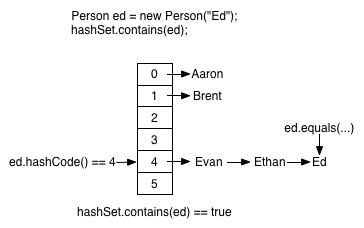
\includegraphics[height=2.5in]{hashtable-find.png}
\end{center}
\vspace{-.1in}
If you override {\tt equals}, you must override {\tt hashCode}!
\end{frame}
%------------------------------------------------------------------------

%------------------------------------------------------------------------
\begin{frame}[fragile]{Consequences of Failing to Override {\tt hashCode}}

\begin{lstlisting}[language=Java]
  Set<Trooper> trooperSet = HashSet<>();
  // ...
  trooperSet.add(new Trooper("Mac", true));

  // Mac is in the set, but we don't find him because we didn't
  // override hashCode().
  System.out.println("\nOops!  Didn't override hashCode():");
  System.out.println("trooperSet.contains(new Trooper(\"Mac\", true))="
                     + trooperSet.contains(new Trooper("Mac", true)));

\end{lstlisting}
prints:
\begin{lstlisting}[language=Java]
Oops!  Didn't override hashCode():
trooperSet.contains(new Trooper("Mac", true))=false
\end{lstlisting}

\end{frame}
%------------------------------------------------------------------------

% %------------------------------------------------------------------------
% \begin{frame}[fragile]{}


% \begin{lstlisting}[language=Java]

% \end{lstlisting}

% \begin{itemize}
% \item
% \end{itemize}


% \end{frame}
% %------------------------------------------------------------------------


\end{document}
